%2.1.tex

RISC-Vはカルフォルニア大学バークレイ校が新たに開発したRISCの設計思想に基づく命令セットアーキテクチャ(ISA)である.RISC-VはオープンなISAであり,ライセンスが不要である.

従来のISAでは,後方バイナリ互換性を維持するために過去に拡張した命令すべてを実装する必要がある.しかし,このようなISAでは命令数が増加し複雑になる.そこでRISC-Vではモジュール式ISAを採用している.\cite{bib:risc-v-module}
RISC-Vのシステムの機能を独立したモジュールとして分け,アプリケーションに応じて拡張機能を組み込むかを選択できる.RISC-Vには必ず組み込まなければならない基本命令セット(RV32I)の他に,主な拡張機能として乗算及び除算(RV32M),単精度浮動小数点(RV32F),倍精度浮動小数点(RV32D)等がある.

RISC-Vの基本命令は6つの命令フォーマットで表すことができる.基本命令の命令フォーマットを図\ref{fig:RISC-V_Instruction_formats}
に示す.

\begin{figure}
    \centering
    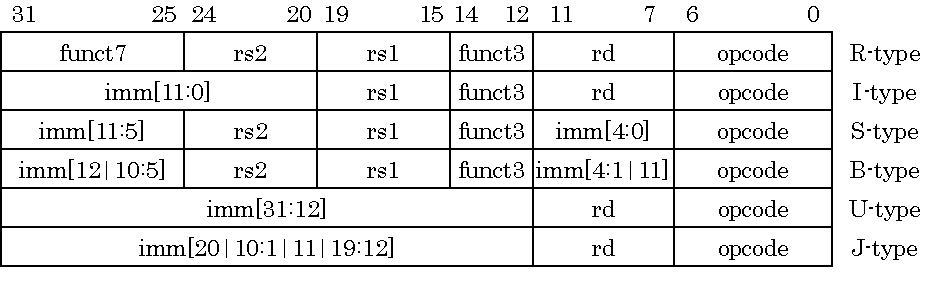
\includegraphics[scale=0.8]{image/Inst_Format.pdf}
    \caption{基本命令の命令フォーマット}
    \label{fig:RISC-V_Instruction_formats}
\end{figure}

R形式は2つのソースレジスタを扱う形式,I形式は12ビットの即値を扱う命令,S形式はストア命令,B形式は条件分岐命令,U形式は20ビットの即値を扱う命令,J形式は無条件ジャンプ命令の形式である.命令形式が単純であるため命令のデコーディングが単純化される.